    \item Let $\vec{A} = \myvec{5 & -3 \\ 6 & -4}$. Then the trace of $\vec{A}^{1000}$ equals
    \hfill{\brak{\text{XE 2018}}}
    \begin{enumerate}
        \begin{multicols}{4}
            \item $2^{1000} - 1$
            \item $2^{1000} + 1$
            \item 1
            \item $2^{1000}$
        \end{multicols}
    \end{enumerate}
    \item A horizontal effort $\vec{P}$ is applied to raise a block of weight $\vec{W}$ on a rough surface inclined at an angle $\theta$ with the horizontal. If $\mu_s$ is the coefficient of static friction between the block and the surface, the minimum effort $\vec{P}$ required to impend the upward motion of the block along the surface is
    \hfill{\brak{\text{XE 2018}}}
    \begin{figure}[H] \centering 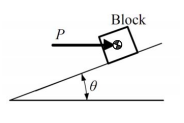
\includegraphics[width=0.4\columnwidth]{GATE/2018/XE/figs/q11_solid.png} \caption{} \label{fig:q11_solid} \end{figure}
    \begin{enumerate}
        \begin{multicols}{4}
            \item $\vec{W} \brak{\frac{\mu_s - \tan\theta}{1+\mu_s\tan\theta}}$
            \item $\vec{W} \brak{\frac{\mu_s + \tan\theta}{1-\mu_s\tan\theta}}$
            \item $\vec{W} \brak{\frac{\mu_s - \tan\theta}{1-\mu_s\tan\theta}}$
            \item $\vec{W} \brak{\frac{\mu_s + \tan\theta}{1+\mu_s\tan\theta}}$
        \end{multicols}
    \end{enumerate}

